\section{Kommunikationsmodelle}
Kommunikationsmodelle beschreiben die wechselseitige Informationsübertragung zwischen den verschiedenen Kommunikationsteilnehmern. Mit diesen werden Prozesse in ihren einzelnen Bestandteilen dargestellt. Die hier in Abbildung \ref{img:deskriptiv} und Abbildung \ref{img:präskriptiv} gezeigten Modelle sind allgemeine Kommunikationsmodelle. Während die Abbildung \ref{img:deskriptiv}: \nameref{img:deskriptiv} den Ist-Zustand veranschaulicht, stellt die Abbildung \ref{img:präskriptiv}: \nameref{img:präskriptiv} den Soll-Zustand dar.\\\\
\begin{figure}[H]
	\centering
	\setlength{\fboxsep}{1pt}
	\setlength{\fboxrule}{1pt}
	\fbox{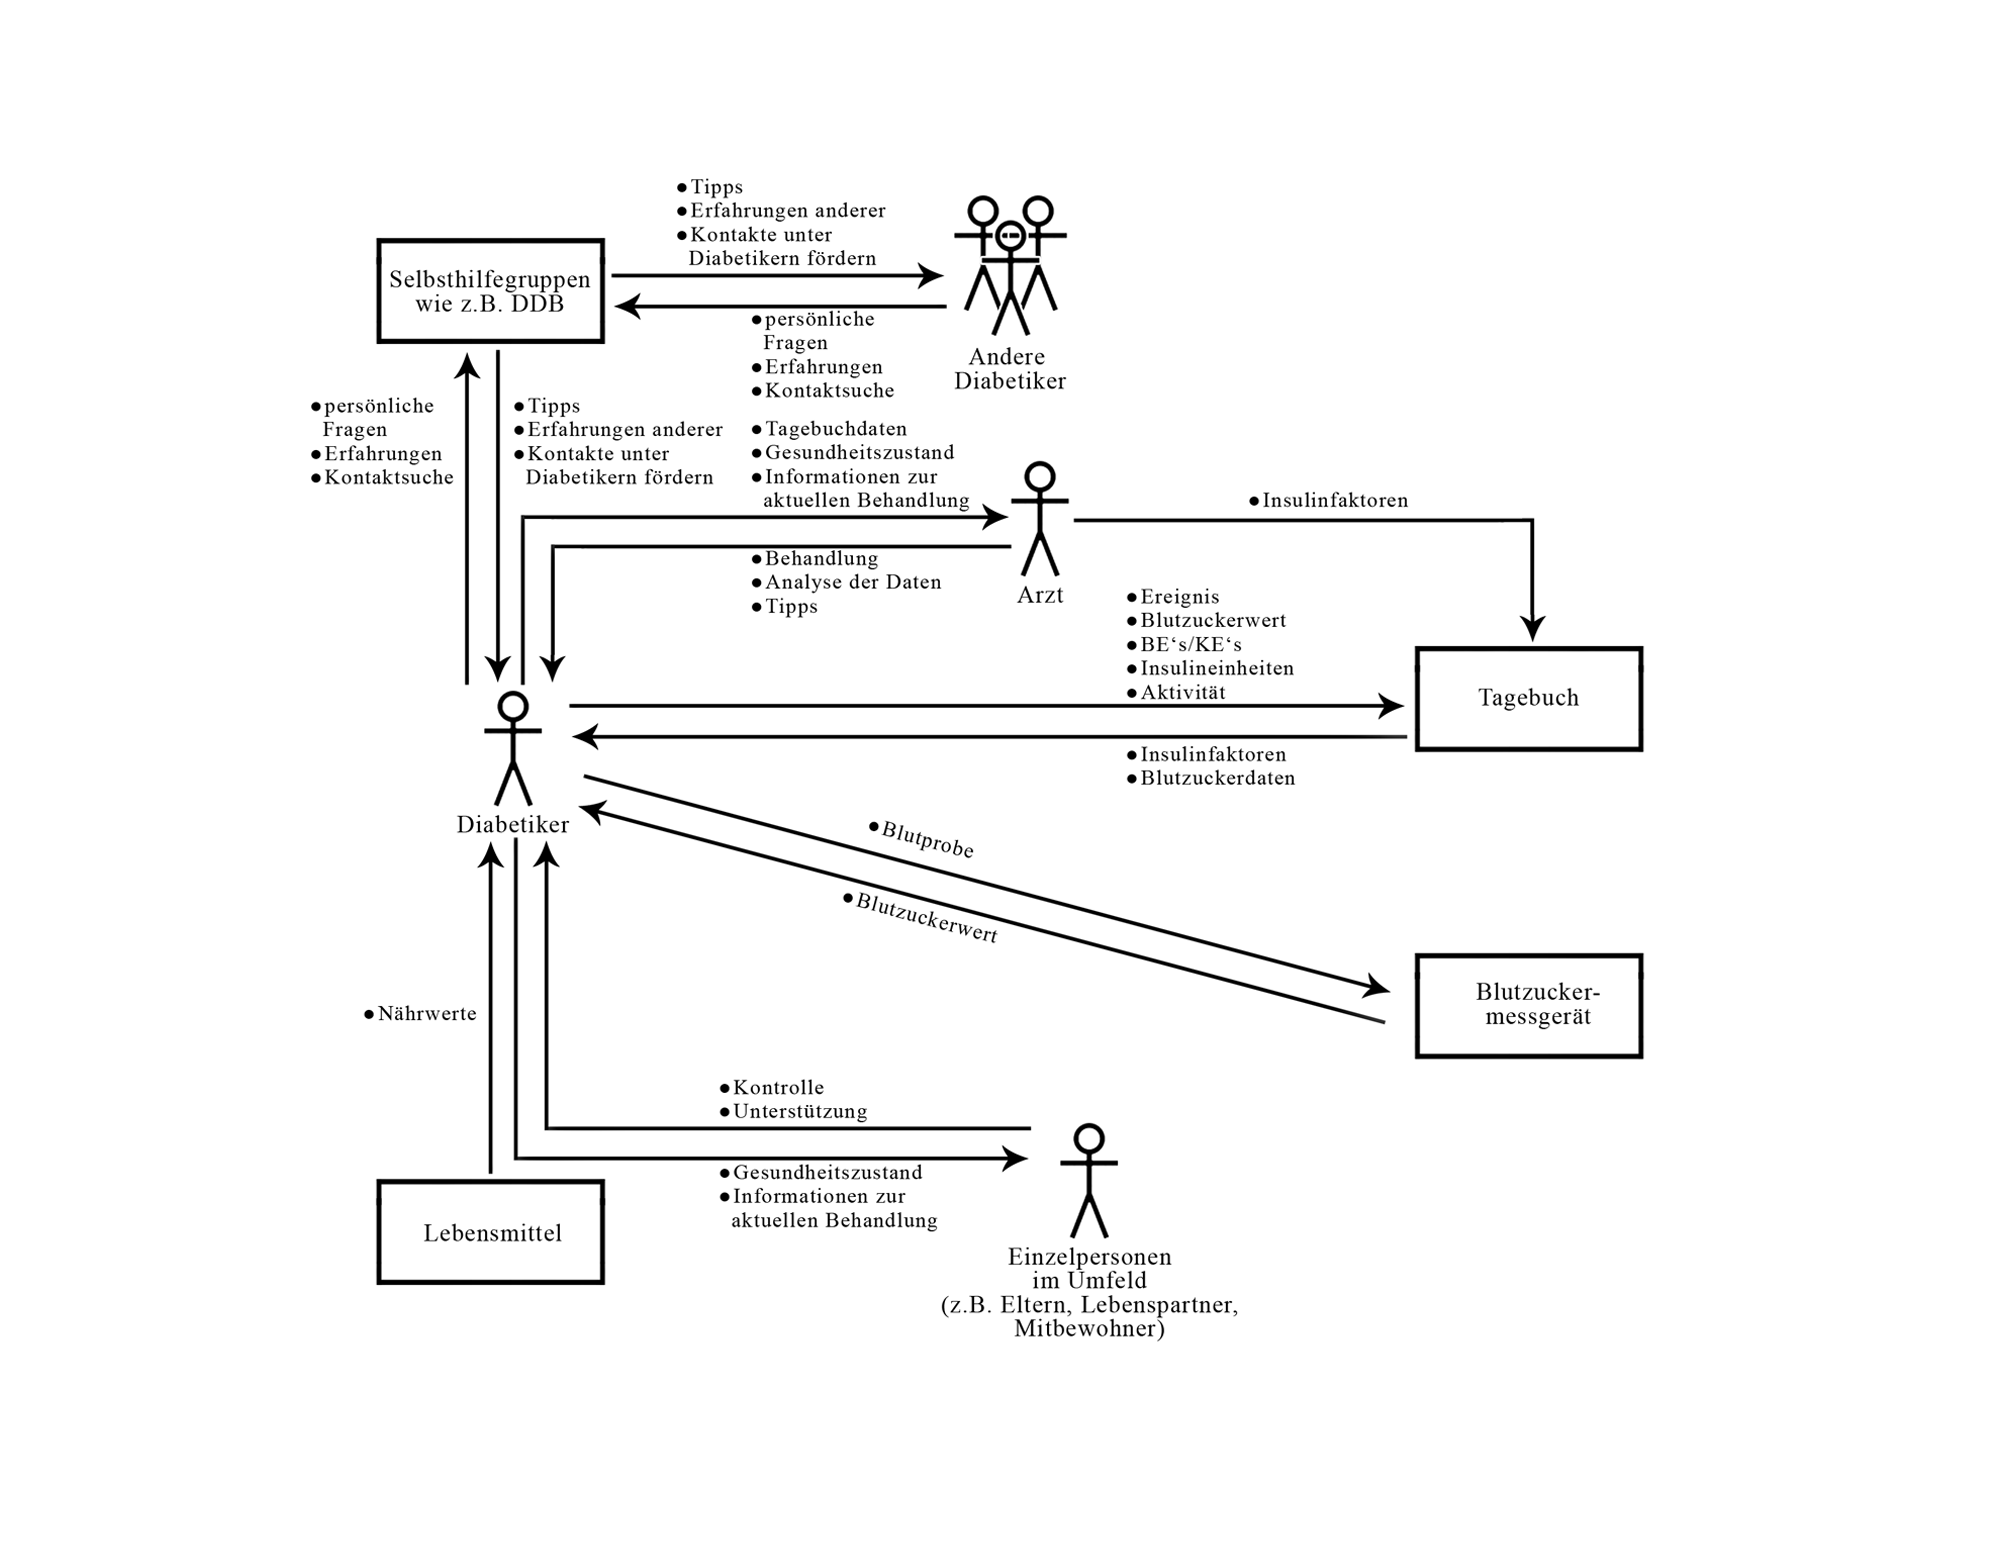
\includegraphics[width=1.0\textwidth]{images/deskriKommDiagramm.png}}
	\captionsetup{justification=centering}
	\caption{Deskriptives Kommunikationsmodell}
	\label{img:deskriptiv}
\end{figure}
\begin{figure}[H]
	\centering
	\setlength{\fboxsep}{1pt}
	\setlength{\fboxrule}{1pt}
	\fbox{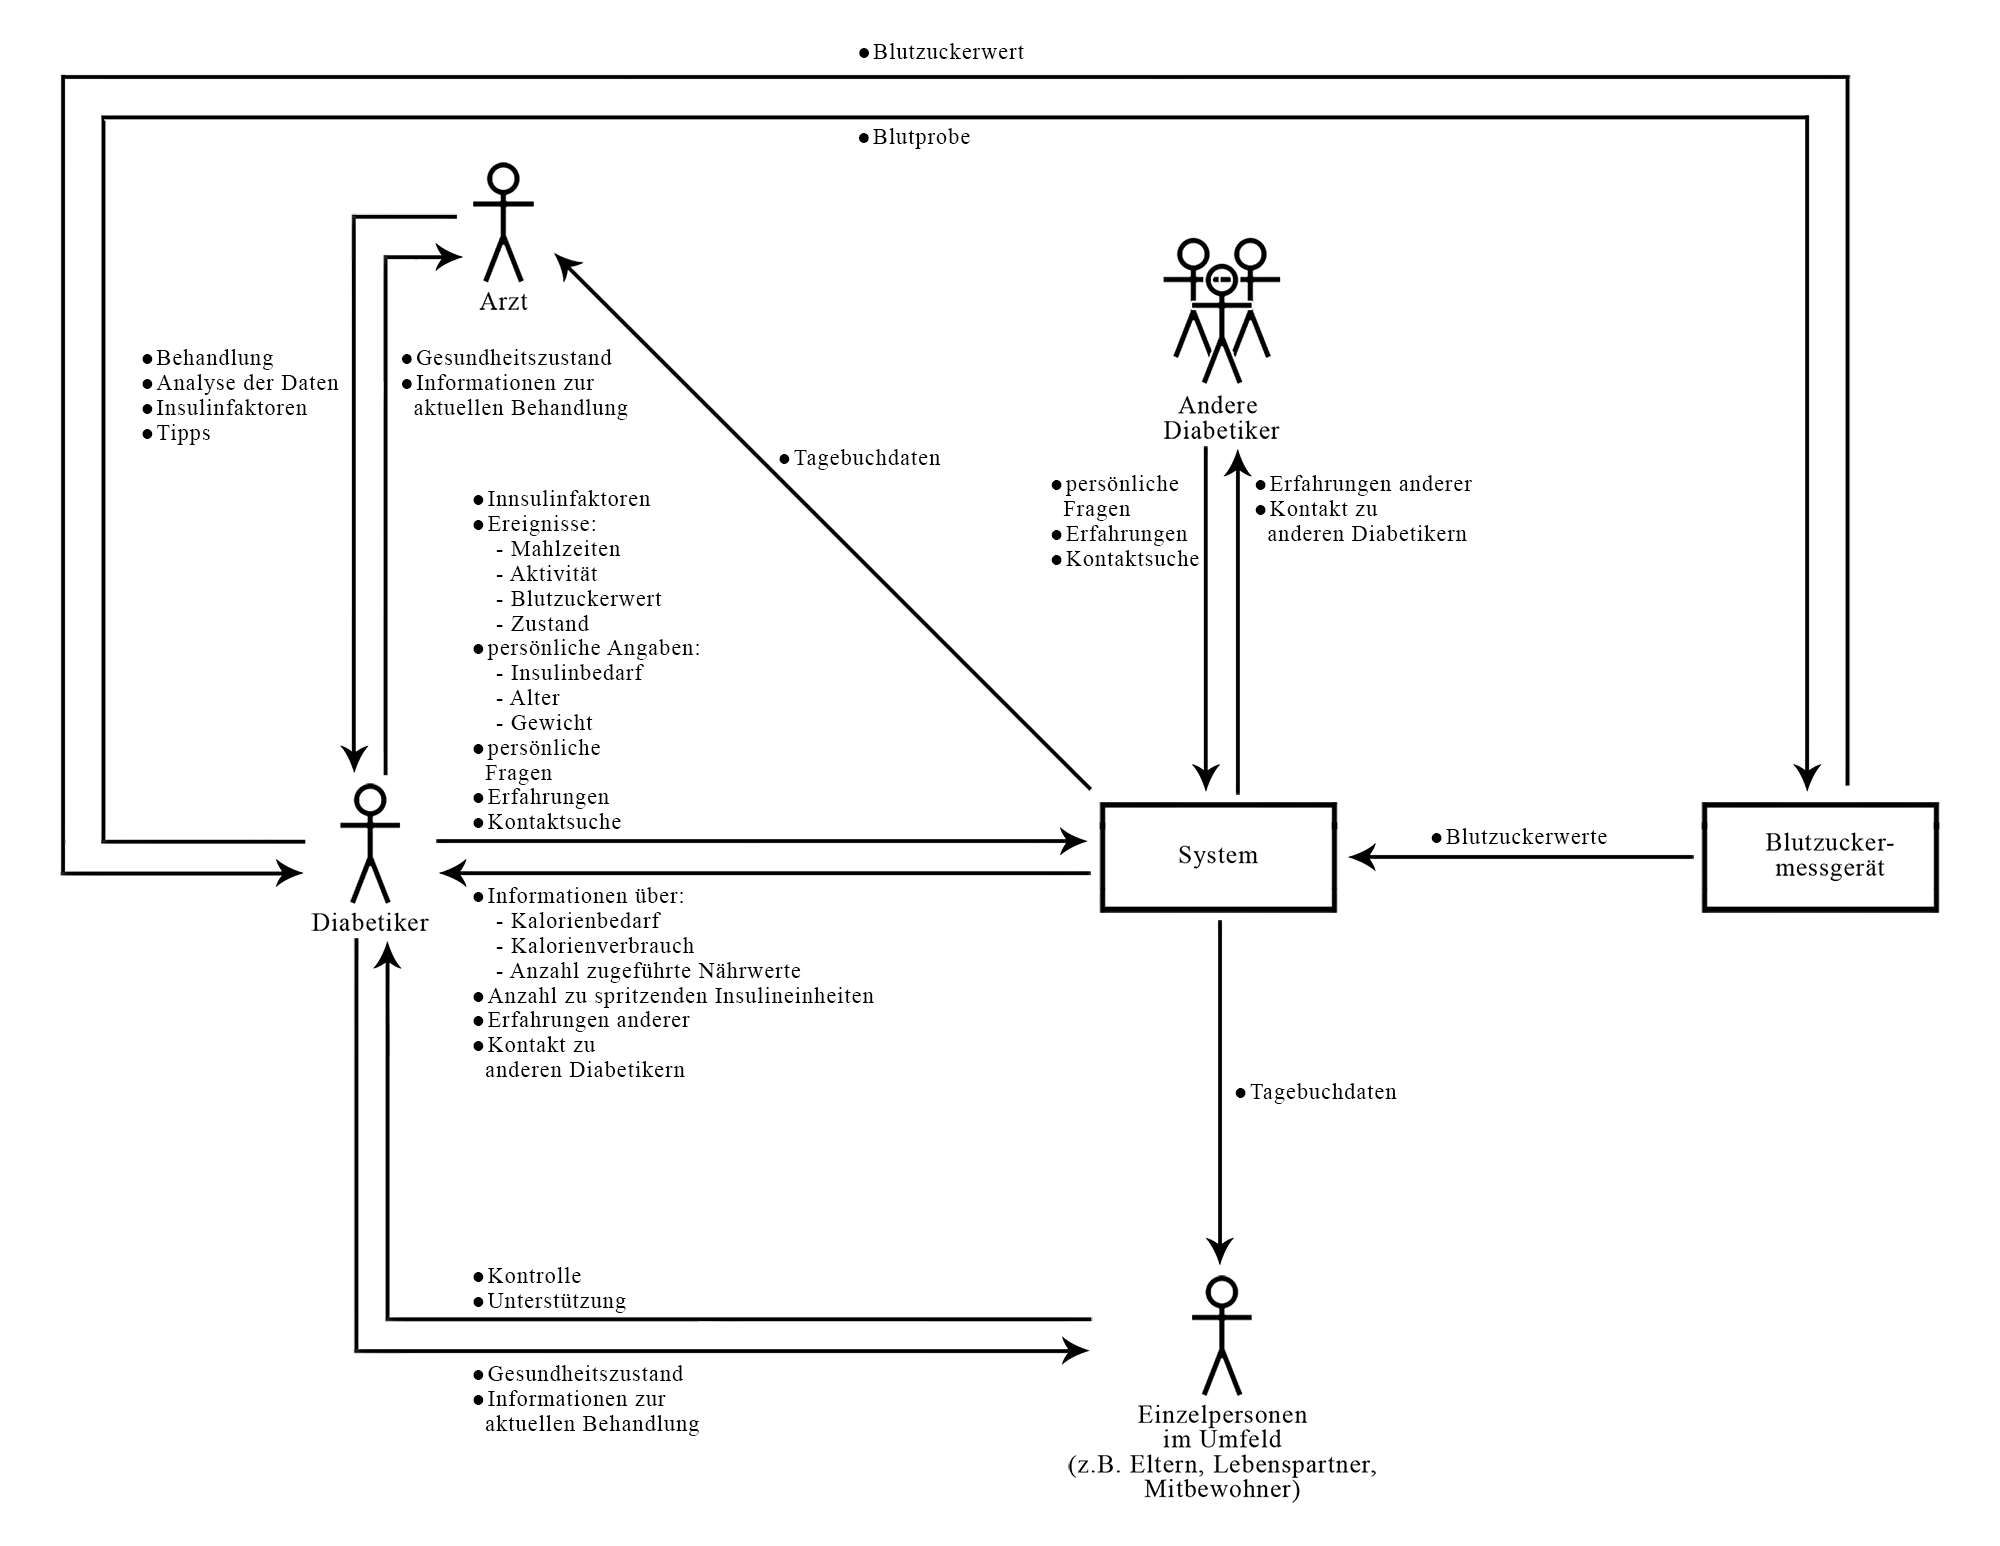
\includegraphics[width=1.0\textwidth]{images/praskriKommDiagramm.png}}
	\captionsetup{justification=centering}
	\caption{Präskriptives Kommunikationsmodell}
	\label{img:präskriptiv}
\end{figure}